\chapter{Introduction}
\label{chapter:intro}


Projection mapping is projecting on anything that is not a projection screen. While screens in cinemas and classrooms are made specifically for being projected onto, this is not the case for other objects, for example building façades. The geometry and material properties of these objects deform projection images and chainge their appearance. This is why projecting them is not enough -- they also need to be \textit{mapped} in a way that their final appearance is what we expect.

\begin{figure}[ht]
    \begin{center}
        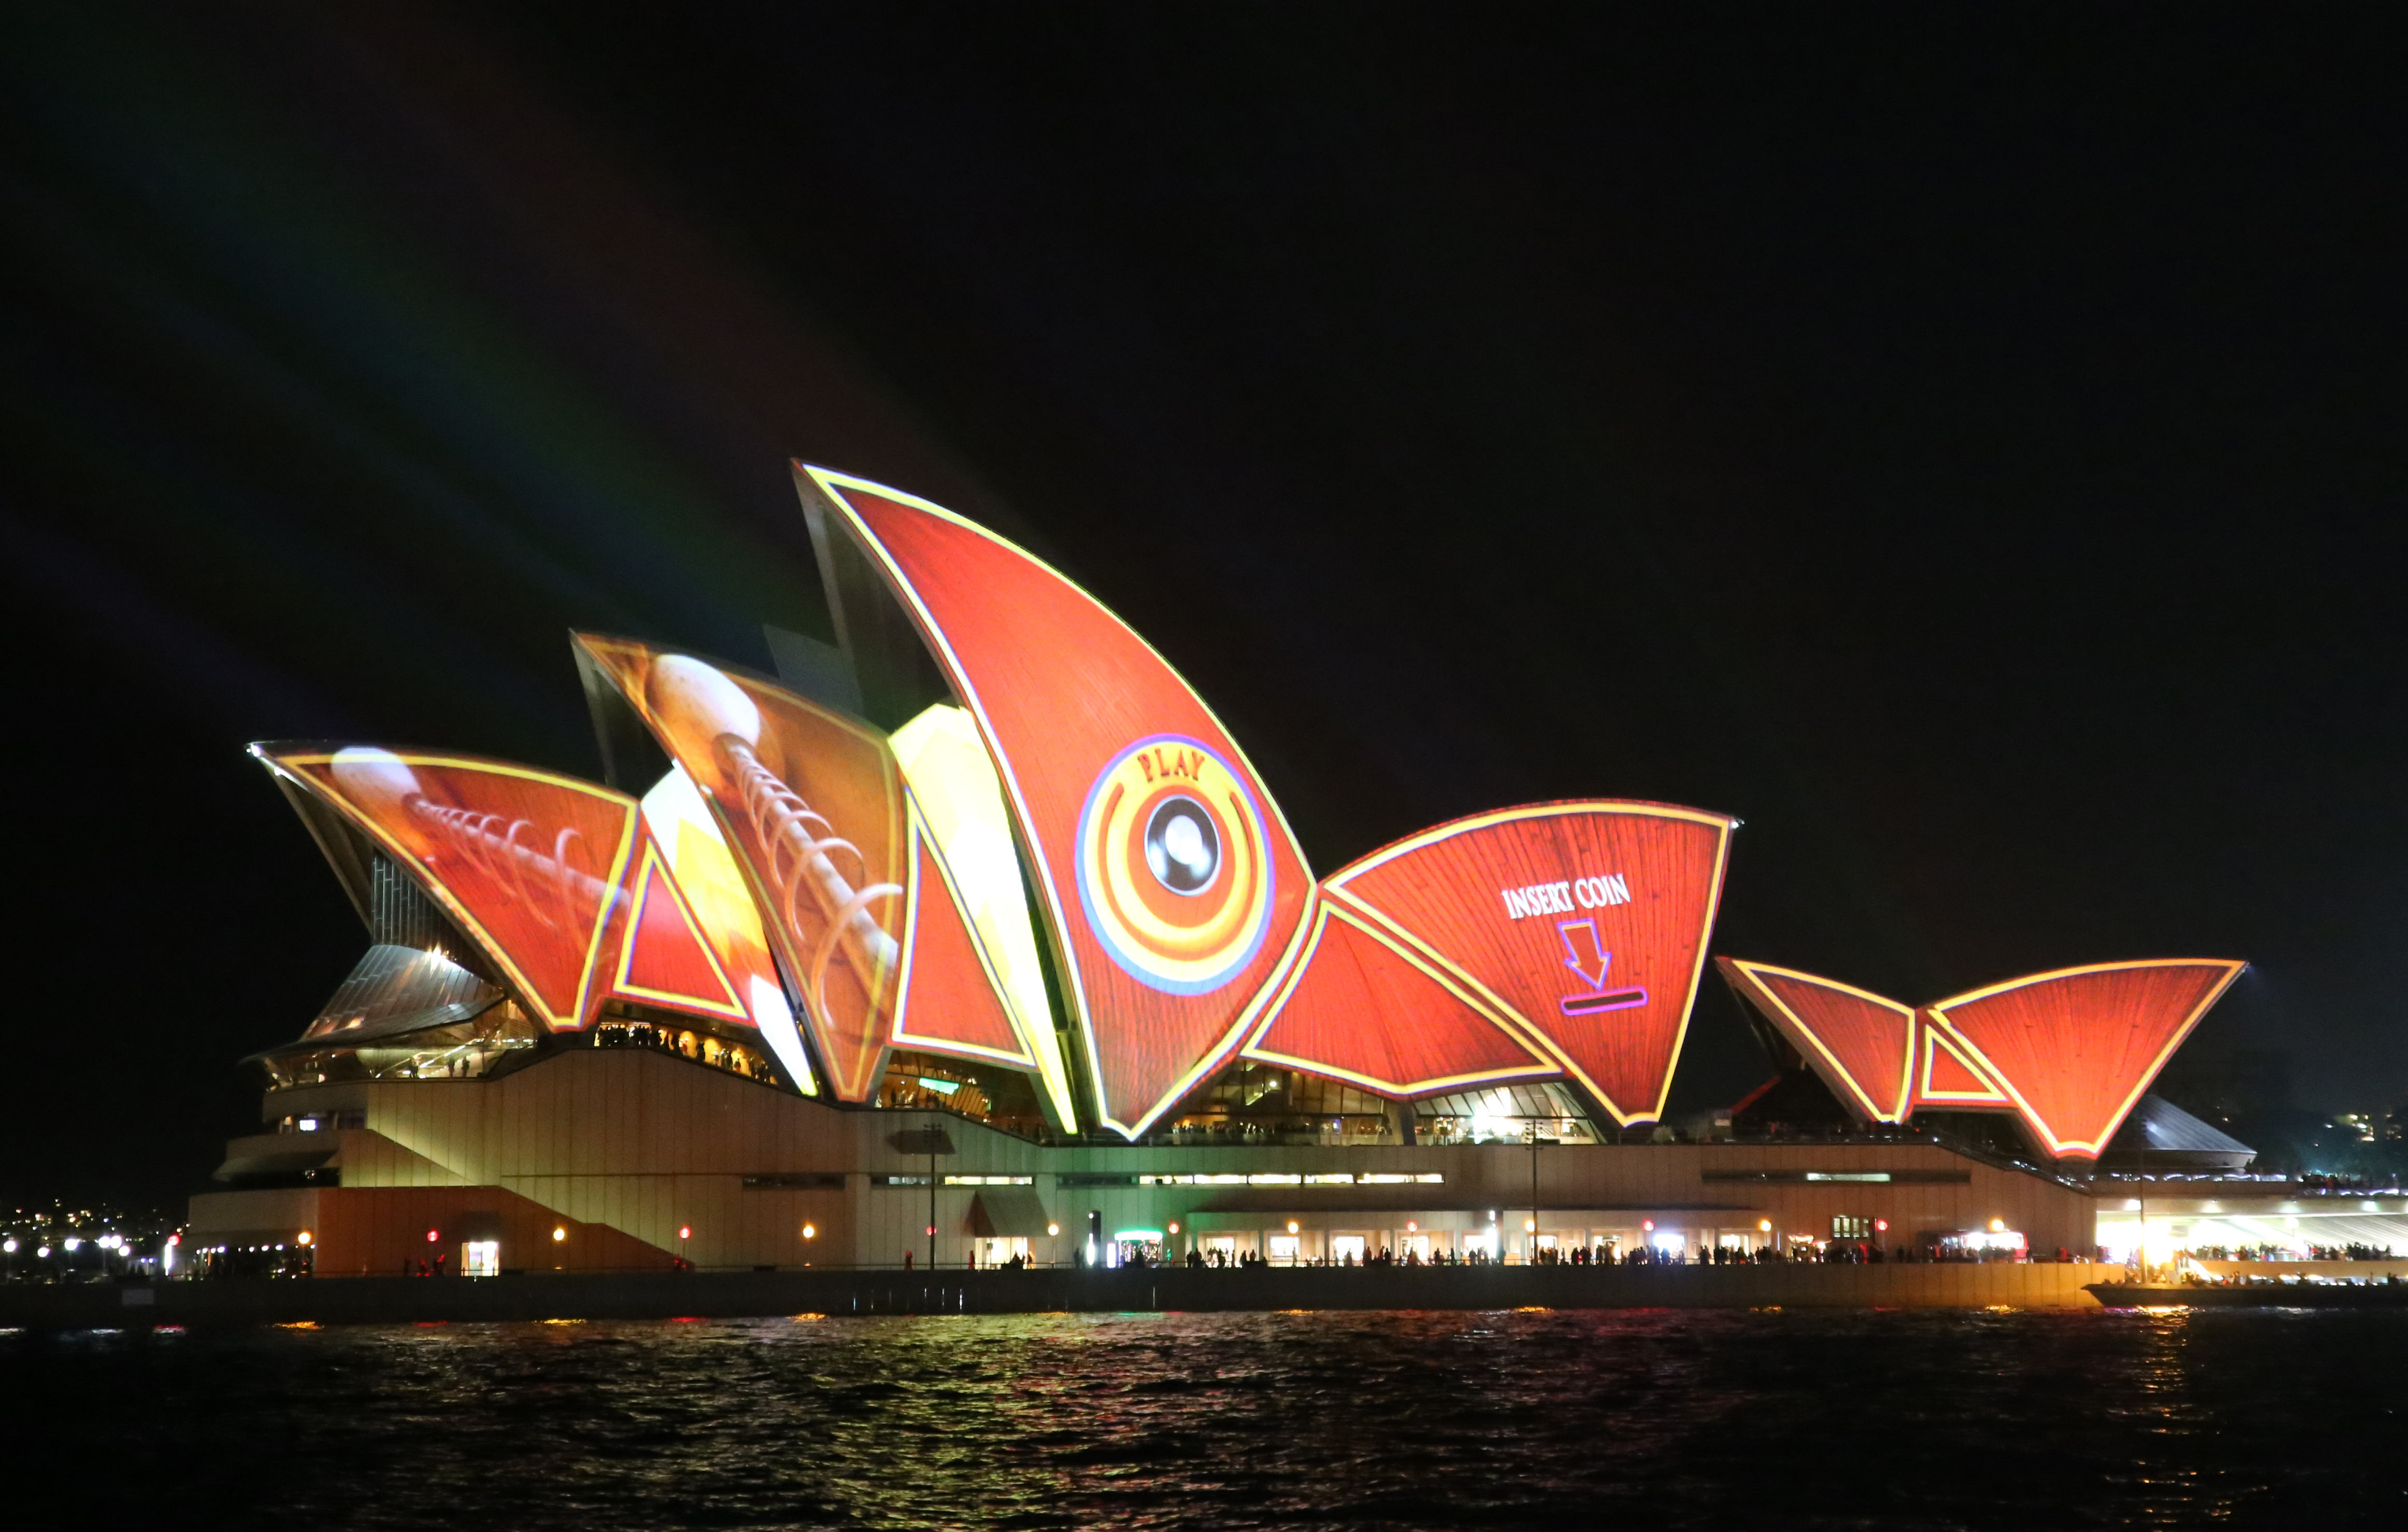
\includegraphics[width=0.8\textwidth]{images/01-projection_mapping_example_sydney.jpg}
        \caption{Source: \citet{ImageProjectionMappingExampleSydney}}
        \label{fig:intro_example_sydney}
    \end{center}
\end{figure}

According to \citet*{WikiHauntedMansion}, one of the first uses of projection mapping (also sometimes called \textit{video mapping} or \textit{spatial augmented reality}) was in The Haunted Mansion Disneyland ride which opened in 1969. There, a video of a human face is projected onto a static head. Projection mapping has become widespread in recent years. It is used to augment reality by artists from all over the world in galleries, museums and outdoor spaces. One prominent example is projection mapping on buildings (see \ref{fig:intro_example_sydney}) which is done in cities during festivals and other special occasions.

\section{Problem Setting}
\label{section:intro-problem_setting}

The usual workflow of projection mapping involves the following steps:

\begin{enumerate}
    \item We have an image we want to project onto a scene. If we do that directly, the appearance will not be what we want because the scene influences our projection in an unpredictable manner
    \item We need to create a \textit{compensated projection image} that will look like our original projection image when projected onto our scene
    \item We project the compensated image
\end{enumerate}

In this thesis, we focus on creating the compensated projection image automatically. There is a wide body of research focusing on this problem. In one of the earliest papers of the field, \citet*{Grossberg2004} project a series of special calibration images onto a scene and capture their appearance using a camera. Using these \text{camera images}, they are able to estimate the parameters of a model that determines how each pixel of the projection influences the appearance in that particular scene. Once this calibration is ready, they are able to compute compensation images on the fly using the model. The combination of a projector and a camera is common in projection mapping and such systems are called \textit{projector-camera systems}.

{\color{red} TODO: figure of the general process}

Since then, there have been many advances in the field which are summarized in a state-of-the-art report by \citet*{Grundhofer2018}. Nowadays, projector-camera systems are able to calibrate themselves automatically after they are placed in a scene and they can also re-calibrate themselves in real time, for example when scene illumination changes, or when objects in the scene are transformed, both rigidly (i.e. without deformation) and non-rigidly. It is worth noting that because of the sheer complexity of general projection mapping, no single method solves this problem completely. For example, methods that handle non-rigid transformations will often rely on object tracking which requires the object to have markers on it. Such methods might also break when illumination changes significantly.

There is, however, one fundamental characteristic that all current projection-mapping methods share. When computing the compensated projection image, they are trying to ensure that the camera image will match the desired appearance pixel by pixel. Explicitly, their goal is

\[
    X = Y
\]

where \(X,Y \in \mathbb{R}^{n \times m}\) are the camera image and desired appearance, respectively.

This approach is limited by projector hardware. Every projector has finite brightness which means that pixels of the camera image cannot be made arbitrarily bright. In scenes with external illumination (which are most scenes -- due to light pollution it is nearly impossible to find complete darkness nowadays), it is also impossible to make pixels of the camera image arbitrarily dark since projectors only add light and do not subtract it.

{\color{red} TODO: figure of the limitation of pixel-by-pixel matching}

In this thesis, we present an idea to overcome this limitation by reformulating what it means that camera image and desired appearance match.

\section{Key Idea of Neural Projection Mapping of Textures}
\label{section:intro-key_idea}

Textures (e.g. a stony beach) have the interesting property that when their features (e.g. individual stones) are shuffled, the texture still looks the same. For example, \citet*{Julesz1995} defines textures as classes of pictures that cannot be discriminated in preattentive vision. These pictures are not the same pixel by pixel, but they \textit{look} the same when we glance over them.

{\color{red} TODO: figure of the main idea}

The projection-mapping method presented in this thesis focuses on project-mapping textures. The main idea is as follows:

\begin{itemize}
    \item We assume a texture which is difficult to project-map onto a given scene because of brightness limitations of the projector
    \item Out of all possible realizations of that texture, we find the one which is the easiest to project-map onto the scene
    \item We find the appropriate compensated projection image for it
\end{itemize}

A separate research field is dedicated to generating different realizations of the same texture, a task which came to be called \textit{texture synthesis}. \citet*{Raad2018} present a state-of-the-art report of texture synthesis methods. Some of these methods derive a statistical representation of textures such that if two pictures share that representation, they are the same texture. Here are some examples of what such a statistical representation can look like:

\begin{itemize}
    \item Pixel values (this is too restrictive because in this case all texture classes contain only a single image)
    \item Average color (this is too loose because in this case each texture class would contain e.g. a constant image of that color)
    \item Power spectrum (a better representation which works well for textures with tiny features and is used for texture synthesis in \citet*{Galerne2011})
    \item Gram matrices of feature activations of a convolutional neural network (a complex representation presented by \citet*{Gatys2015} which significantly increased the quality of texture synthesis and spurred a wave of new research in the area, including this thesis)
\end{itemize}

{\color{red} TODO: figure to illustrate statistical representations}

We build on these statistics-based synthesis methods and reformulate the goal of projection mapping as follows:

\[
    f(X) = f(Y)
\]

where \(X,Y \in \mathbb{R}^{n \times m}\) are again the camera image and desired appearance, respectively, and \(f\) is a function that assigns a statistical representation to an image.

Provided that our \(f\) describes textures well and an algorithm exists that for a given \(Y\) find an \(X\), so that \(f(X) = f(Y)\), this way of formulating the problem is strictly better than the original per-pixel formulation. This is because \(X = Y\) implies \(f(X) = f(Y)\) and therefore the solution to the original formulation is also a solution to our formulation. On top of that, however, our formulation also has other solutions.

\section{Research Question}
\label{section:intro-research_question}

The ultimate goal of our research is to find a method of projection-mapping textures that achieves higher image quality in challenging conditions than any current method. We have presented a theoretical formulation of the projection-mapping problem that allows for such a method to exist. In this thesis, we explore three questions that will enable us to get closer to the ultimate goal:

\begin{enumerate}
    \item Can we find an algorithm that will give us textures that both match the statistical representation of our target and are easy to project-map?
    \item With known statistical representations, how does such an algorithm compare to per-pixel project mapping?
    \item How practical is this algorithm? Can we deploy it in a projector-camera system?
\end{enumerate}

\section{Neural Projection Mapping of Textures}
\label{section:intro-neural_projection_mapping}

{\color{red} TODO: briefly explain our pipeline (via a figure?):
    \begin{itemize}
        \item Rendering function instead of a real projector-camera system
        \item Computing CNN-based statistics
        \item Comparing them to those of the desired appearance
        \item Driving an optimization process this way
    \end{itemize}
}

{\color{red} TODO: briefly present one interesting result:
    \begin{itemize}
        \item Just a single target-scene-compensation-appearance combo
        \item Introduces the terminology and how the figures are organized
    \end{itemize}
}

{\color{red} TODO: this thesis is organized as follows...}
